% Abschnitt: Besonderheiten 
\section{Besonderheiten}
\label{sec:implementierung:besonderheiten}

\subsection{Wartezeit berechung und -darstellung}
\label{sec:implementierung:besonderheiten:wartezeit}

Für einen möglichst guten Überblick über die Wartezeiten einer Attraktion gibt es in unserer App verschiedene Varianten, wie der jeweilige Durchschnitt und die aktuelle Wartezeit angezeigt wird. Die verschiedenen Arten von Wartezeiten haben wir bereits in Kapitel \ref{sec:grundlagen:bewertugnen} erklärt. In diesem Abschnitt möchten wir noch einmal kurz auf die Art der Berechnung der verschiedenen Wartezeiten eingehen. 

Wir beginnen mit der Erklärung der Wartezeiten, wie sie in der Attraktionsdetail-Ansicht auf Abbildung \ref{figure:implementierungattraktionsansicht} zu sehen sind. Am einfachsten ist sicherlich der Gesamtdurchschnitt der Wartezeiten einer Attraktion. Dieser ist ganz einfach der Durchschnitt aller eingetragenen Wartezeiten seit die Attraktion erstellt wurde, ohne irgendwelche Einschränkungen. Auch der Tagesdurchschnitt ist nicht besonders kompliziert. Er zeigt den Durchschnitt aller bereits am aktuellen Tag eingetragenen Wartezeiten für die Attraktion an. Falls am aktuellen Tag noch keine Wartezeit für eine Attraktion eingetragen wurde, wird jeweils der Tagesdurchschnitt für den letzten Tag angezeigt, an dem eine Wartezeit eingetragen wurde. Zudem wird der Tag der letzten Aktualisierung mit angegeben. Die aktuelle Wartezeit wird derzeit als Durchschnitt der letzten drei eingetragenen Wartezeiten berechnet. Der Grund hierfür ist, dass einer einzelnen Wartezeit nicht zu viel Gewichtung gegeben werden soll, um so die Auswirkungen einer möglichen falsch eingetragenen Wartezeit zu verringern.

Für einen schnellen Überblick sind die Wartezeiten auch durch Farben gekennzeichnet. Dabei entspricht die Farbe grün, dass wenig los ist, gelb dass mittel viel los ist und rot dass viel los ist. Alle drei Wartezeiten auf der Attraktionsdetail-Ansicht sind grün, wenn sie jeweils unter 10 Minuten liegen und rot, falls sie über 90 Minuten liegen. Zudem gilt für die Aktuelle Wartezeit und für den Tagesdurchschnitt, dass sie grün sind, falls sie weniger als 70 Prozent des Gesamtdurchschnitts entsprechen und rot, falls sie mehr als 130 Prozent des Gesamtdurchschnitts betragen. In allen anderen Fällen sind sie gelb. 

Die letzte Ansicht von Wartezeiten in der Attraktionsdetail-Ansicht ist ein Säulendiagramm, welches die duchschnittlichen Wartezeiten je nach Uhrzeit angibt. Dabei wird für alle Uhrzeiten zwischen 8 Uhr morgens und 20 Uhr der Durchschnitt aller Wartezeiten berechnet. Die anderen Uhrzeiten werden außen vor gelassen, da zu diesen Uhrzeiten kaum Freizeitparks geöffnet haben. Eine Wartezeit, welche zum Beispiel um 11:30 Uhr eingetragen wird, fällt somit in die Stunde zwischen 11 Uhr und 12 Uhr und wird im Diagramm in die Berechnung für die Säule "11"  miteinbezogen.

In der Attrakionsübersicht, wie sie in Abbildung \ref{figure:implementierungattraktionsuebersicht} zu sehen ist, wollen wir dem Nutzer einen schnellen Überblich über die Attraktionen und insbesondere über die aktuelle Wartezeit verschaffen. Um eine möglichst gute Live-Statistik der Wartezeiten mit den aktuellsten Wartezeiten anzubieten, gibt es hier eine leicht abgewandelte Berechnungsmethode. Im allgemeinen wird auch hier der Durchschnitt der letzten drei eingetragenen Wartezeiten verwendet. Gibt es aber an einem Tag bisher weniger als drei Wartezeiten, so wird nur der Durchschnitt dieser angezeigt. Sollte an einem Tag noch gar keine Wartezeit eingetragen sein, dann wird der Tagesdurchschnitt des letzten aktualisierten Tages angezeigt. Die Wartezeiten sind auch hier wieder, wie oben erklärt, farblich gekennzeichnet und zudem wird die Uhrzeit oder der Tag der letzten Aktualisierung mit angegeben. Sollte eines Tages eine Einbindung von Live-Wartezeiten über eine fremde API eines Freizeitparks geschehen, wäre diese Liste der Ort, an welchem sie eingebunden werden könnten.

Generell werden die Wartezeiten in der App von den Benutzern eingetragen. Damit ein Nutzer die Wartezeiten eintragen kann, müssen zunächst drei Bedingungen erfüllt sein:
\begin{enumerate} 
\item Der Nutzer muss mit seinem Account eingeloggt sein. Nur so kann sicher gestellt werden, dass die Funktion nicht missbraucht wird oder ein Nutzer sehr viele Wartezeiten hoch lädt und somit den Durchschnitt manipuliert.
\item Der Nutzer muss sein GPS eingeschaltet haben und sich in einem bestimmten Umkreis zum Park befinden. Das stellt sicher, dass auch wirklich nur Nutzer Wartezeiten eintragen können, die sich auch wirklich im Park befinden.
\item Der Nutzer darf in der letzten Stunde keine Wartezeit eingetragen haben. So soll sicher gestellt werden, dass nicht ein Nutzer die Funktion missbraucht und viele Wartezeiten hoch lädt. Zudem kann angenommen werden, dass sich die Wartezeit nicht ständig ändert und ein stündlicher Intervall für das Eintragen genügt.
\end{enumerate}

Hat ein Nutzer alle Bedingungen erfüllt, wird seine neue Wartezeit eingetragen. Damit nicht jedes Mal erneut alle Durchschnitte berechnet werden müssen, wenn eine Attraktion aufgerufen wird, werden alle oben genannten Durchschnitte sofort nach dem Eintragen berechnet und abgespeichert. So müssen jeweils nur noch die Werte ausgelesen werden. Damit die Berechnung nicht unnötige Rechenleistung auf dem Server verbraucht, passiert diese bereits beim Client und die neu berechneten Werte werden dann auf den Server hochgeladen. Bekanntlich kann diese Art der Aktualisierung möglicherweise zu der Lost-Update-Anomalie führen, falls zwei Nutzer zu dem exakt selben Zeitpunkt eine Wartezeit eintragen. Dies hat aber in diesem Fall keine negative Auswirkung, da ja zum selben Zeitpunkt auch die eingetragene Wartezeit die selbe sein sollte.

\subsection{Client-Server-Kommunikation mit Azure}
\label{sec:implementierung:besonderheiten:azure}

Für die Speicherung der Daten haben wir uns entschieden, den Dienst Microsoft Azure auszuprobieren. Dieser stellt verschiedene hilfreiche Dienste zur Verfügung, welche wir mit einem Studentenaccount kostenlos nutzen können. Zum einen wird ein Server für die Speicherung von Daten zur Verfügung gestellt. Und dazu kommt auch gleich noch eine darauf laufende Datenbank, in unserem Fall SQLite mit node.js, auf der alle primitiven Datentypen gespeichert werden und auch online im Portal eingesehen werden können. Desweiteren kann direkt für Mobile-Projekte auch auf eine kompakte Version von den Diensten namens Microsoft Azure Mobile Services zurückgegriffen werden. Auch eine verschlüsselte Verbindung ist mit Microsoft Azure gewährleistet.

Für unser Projekt brauchen wir nur einen geringen Teil aller Dienste, die Microsoft Azure anbietet. Wir verwenden es ausschließlich zum persistenten Speichern von Daten in einer Datenbank sowie zum schnellen Auslesen und Eintragen. Das haben wir auch nochmal in einem Model in Abbildung \ref{figure:besonderheitenAzure} zusammengefasst.

%Download- und Upload-Verlauf-Modell
\begin{figure}[htp]
	\centering
  	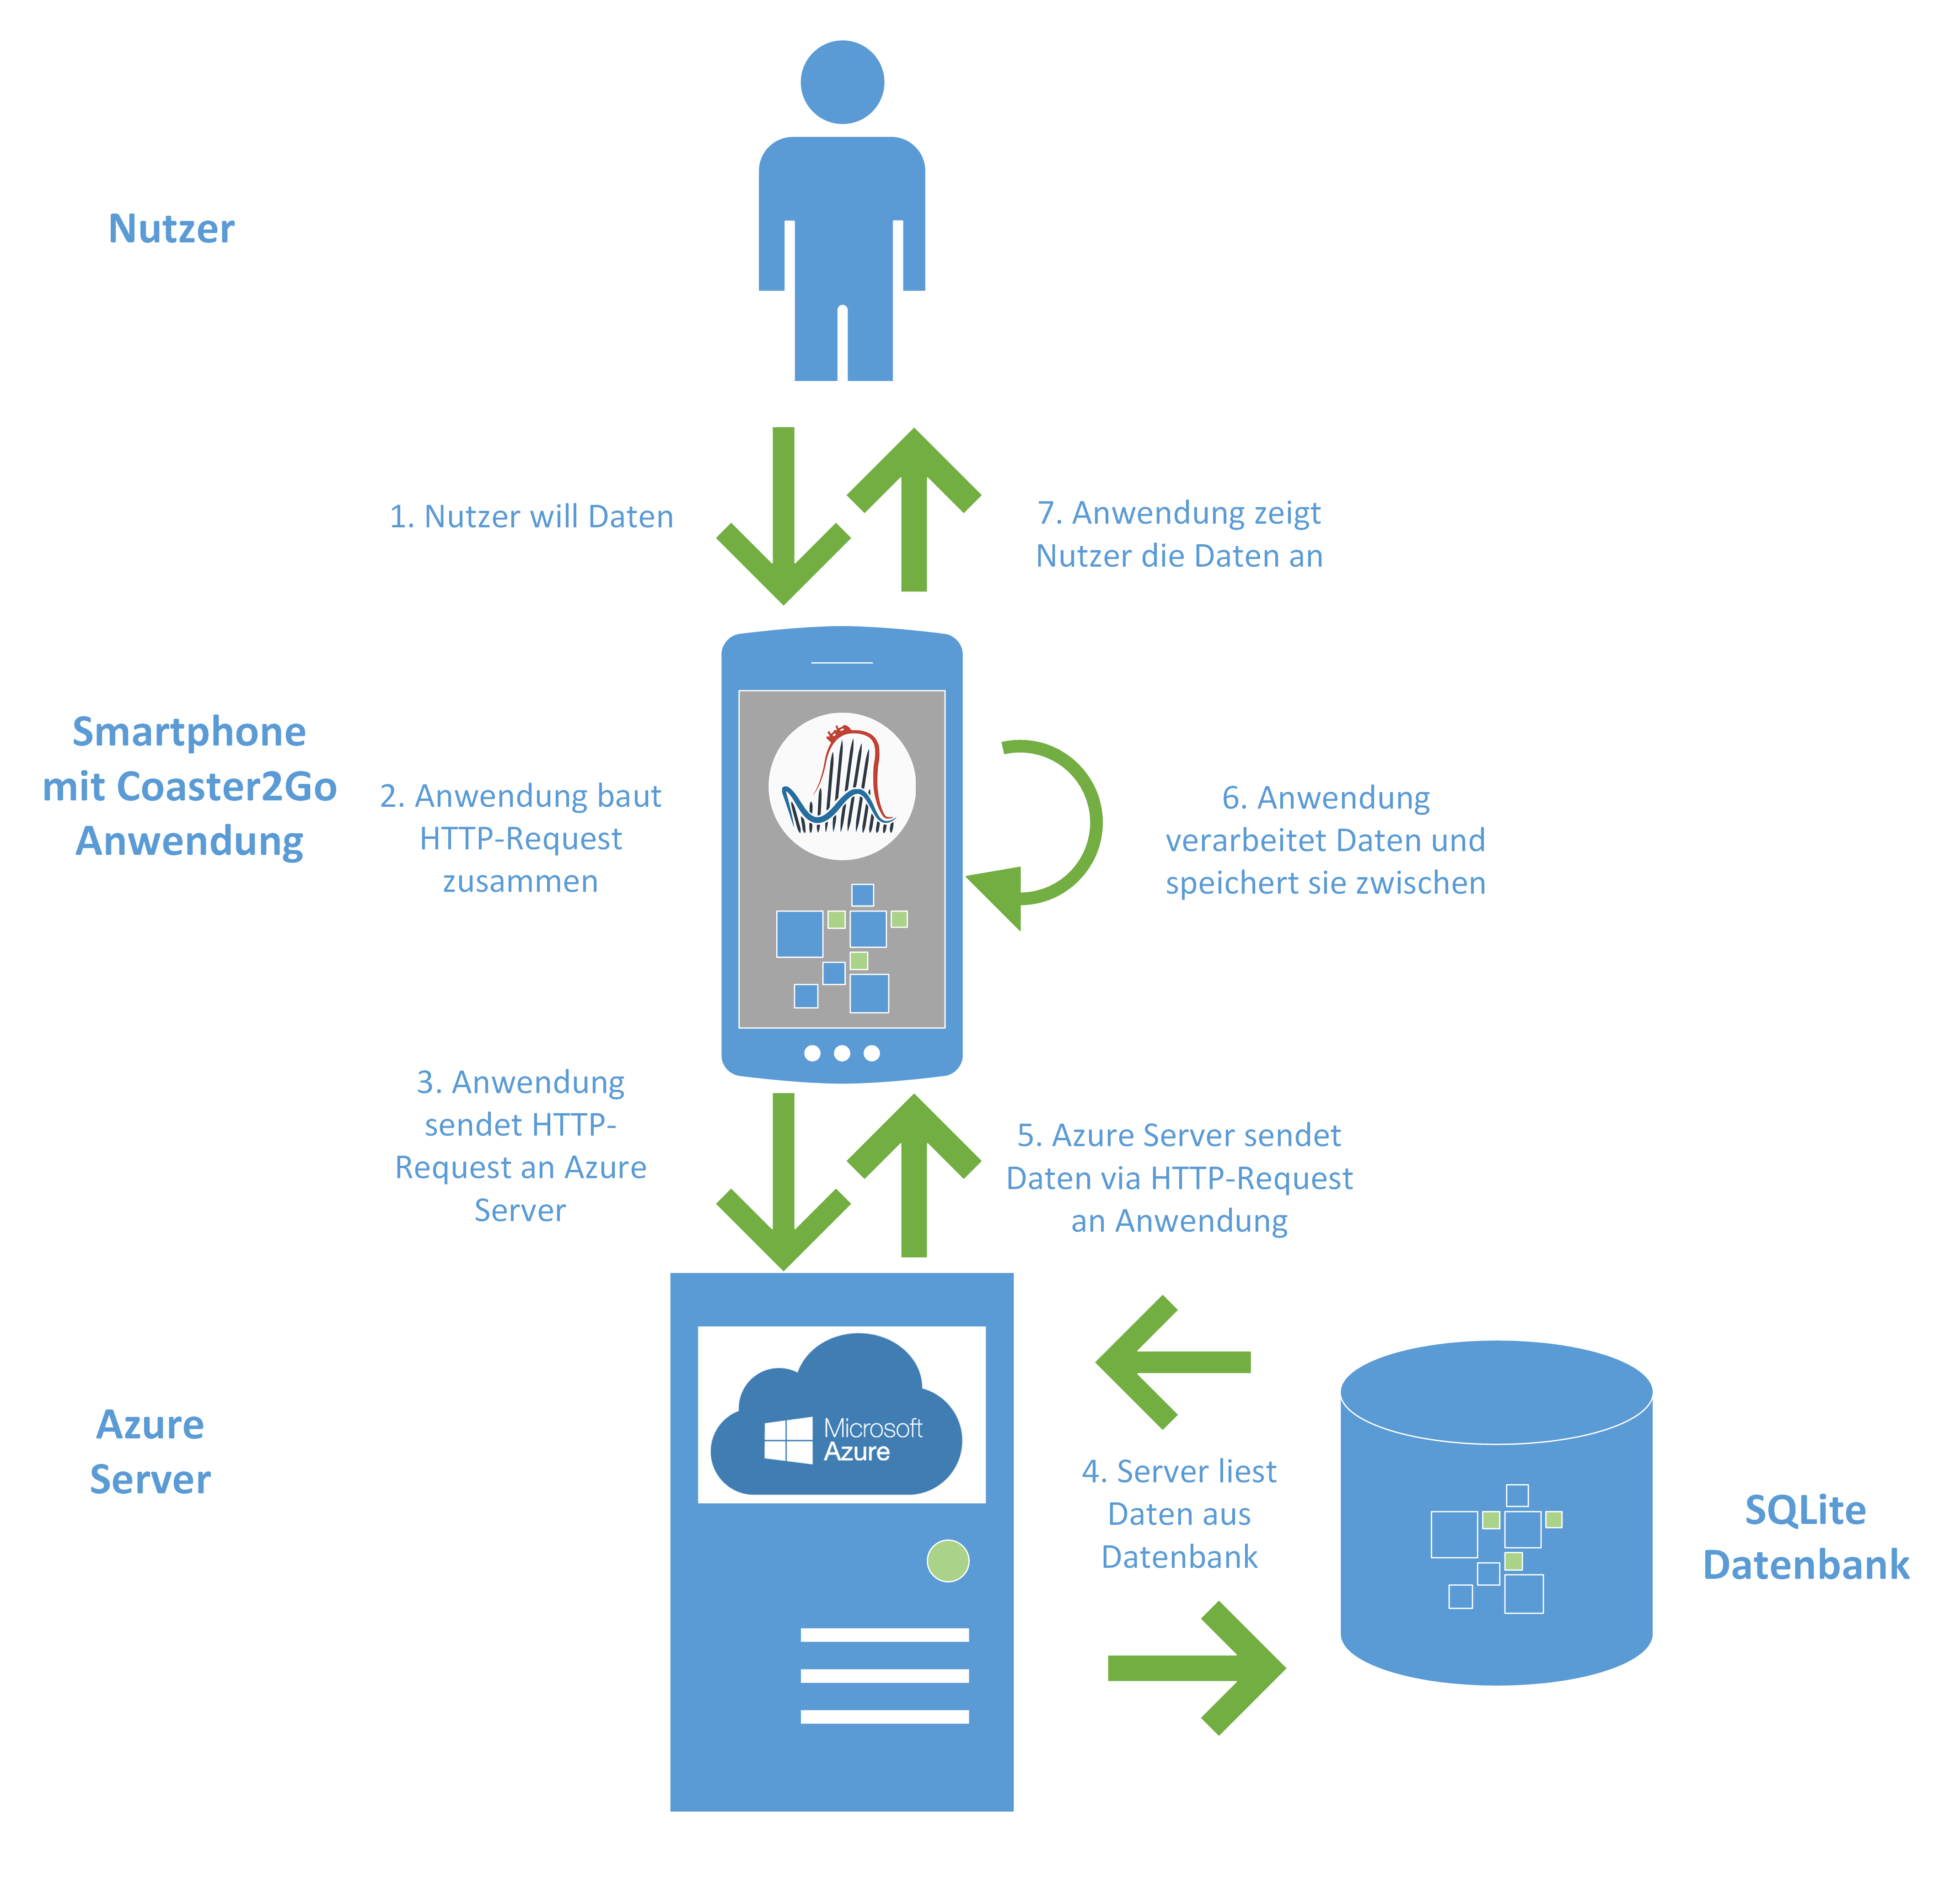
\includegraphics[width=0.99\textwidth]{img/modelle/azure_downloadmodell.png}
	\caption{Azure Daten Download Modell}
	\label{figure:besonderheitenAzure}
\end{figure}

Der Service von Microsoft bietet viele Vorteile. Zum einen ist da natürlich die Einfachheit und die gute Kontrolle über die Verwaltung der Daten durch das Online-Portal zu nennen. Auch das Zusammentreffen vieler Dienste kann als Vorteil gesehen werden. Mögliche Nachteile sind, dass manchmal die Verbindung zum Azure Server sehr langsam ist und dass man gerade als Student sehr viele Begrenzungen der Dienste in Anspruch nehmen muss.

Gerade aus dem Grund, dass die Verbindung zu Azure eine gute Internetverbindung voraussetzt und wir auch generell in unseren Nichtfunktionalen Anforderungen definiert haben, dass die Anwendung möglichst auch offline genutzt werden soll, speichern wir die wichtigsten Daten für die Anwendung zwischen. Genauer gesagt werden die Freizeitparks, und die dazu gehörigen Attraktionen jedesmal im Hintergrund zwischen gespeichert, wenn ein Nutzer diese runter lädt. Somit köönnen auch alle relevanten Informationen zu den bereits angesehenen Freizeitparks und Attraktionen inklusiver der Wartezeiten auch ohne Internetverbnindung angesehen werden. Falls keine gute Internetverbindung besteht oder die Verbindung zu lange dauert, können somit auch die Offline-Daten angezeigt werden, bis die aktuellen Daten herunter geladen wurden, damit der Nutzer nicht vor einem leeren Bildschirm auf die Daten warten muss. Um den Nutzer zudem vor unnötigen Datanabfragen vom Server zu schützen, werden die Daten auch bei wiederholtem Abfragen innerhalb kürzerer Zeitrräume direkt offline geladen und gar nicht erst eine Anfrage an den Server geschickt. Nicht offline gespeichert werden im Gegensatz dazu Daten, die nicht zwangsweise für die Funktion der App notwendig sind, wie zum Beispiel die Liste von einzelnen Wartezeiten und Bewertungen. Bilder werden nicht offline gespeichert aber gecached, so können sie auch offline angezeigt werden und müssen nicht jedesmal erneut herunter geladen werden, solange das Betriebssystem den Speicherplatz nicht für etwas anderes benötigt.

\subsection{Nutzerverwaltung mit Firebase}
\label{sec:implementierung:besonderheiten:firebase}

Generell wird für das Benutzen unserer App kein Nutzeraccount benötigt. Jegliche Informationen können auch ohne einen eigenen Account eingesehen werden. Bisher wird ein Account nur für zwei Aktionen benötigt: das Eintragen von Bewertungen und das Eintragen von Wartezeiten. Bei beidem soll der Account zum einen vor Missbrauch schützen und zum anderen die Nutzer eindeutig identifizieren. Hinzu kommen noch die Adminfunktionen. Um Parks verwalten zu können, kann ein Nutzer Administrator von einem Park werden. Dieser Nutzer hat dann einige weitere Funktionen, welche den Park betreffen, wie das Bearbeiten der Funktionen und Bilder des Parks, das Hinzufügen und Bearbeiten von Attraktionen zu diesem Park und das Zensieren von anstößigen Bewertungstexten. Während der Testphase der App kann jeder Nutzer einen eigenen Park erstellen und Administrator davon werden.

Da wir eine sehr einfache Nutzerverwaltung haben und neben einem Displaynamen nur die Email und ein Passwort benötigen, wäre es keine Schwierigkeit gewesen, eine eigene Nutzerverwaltung zu schreiben. Der Grund, warum wir dennoch auf einen Fremddienst für die Nutzerverwaltung zurückgegriffen haben ist, dass wir dem Nutzer den Aufwand erleichtern wollen und ihm auch eine Anmeldung mit einem bereits vorhandenem Konto eines Social Media Dienstes ermöglichen wollen. Da es ein großer Aufwand wäre, diese für jeden Dienst einzeln einzubinden, haben wir uns dafür entschieden, die Nutzerverwaltung mit einem Dienst zu realisieren, welcher viele verschiedene Social Media Accounts gemeinsam verwalten kann. In unserem Fall fiel die Wahl auf Firebase.

Firebase, welches mittlerweile zu Google gehört, bietet eine Reihe an Funktionen wie Datenverwaltung, Datensynchronisation oder Nutzerverwaltungen. Für uns war lediglich letzteres relevant. Durch die Einbindung von Firebase in unsere App ist es den Nutzern nun möglich, sich direkt mit ihrem Facebook oder Google Account einzuloggen und die App zu benutzen. Nach der Authentifizierung über den Fremddienst verknüpft Firebase automatisch einen Account unserer App mit dem jeweiligen Account des Fremddienstes. Diesen Vorgang haben wir auch noch einmal in einem Modell in Abbildung \ref{figure:besonderheitenFirebase} zusammengefasst. Desweiteren kann natürlich auch ein neuer Account über eine Emailadresse angelegt werden. Ist ein Nutzer eingeloggt, bliebt er so lange auch nach Beenden der App eingeloggt, bis er sich wieder ausloggt und sich dann erneut direkt mit seinem Account einloggen kann. Um die Privatsphäre einer Person zu schützen, ist es zudem möglich, den Namen, welcher den anderen Nutzern angezeigt wird, zu ändern, damit zum Beispiel nicht der echte Name verwendet wird.

%Firebase Modell
\begin{figure}[htp]
	\centering
  	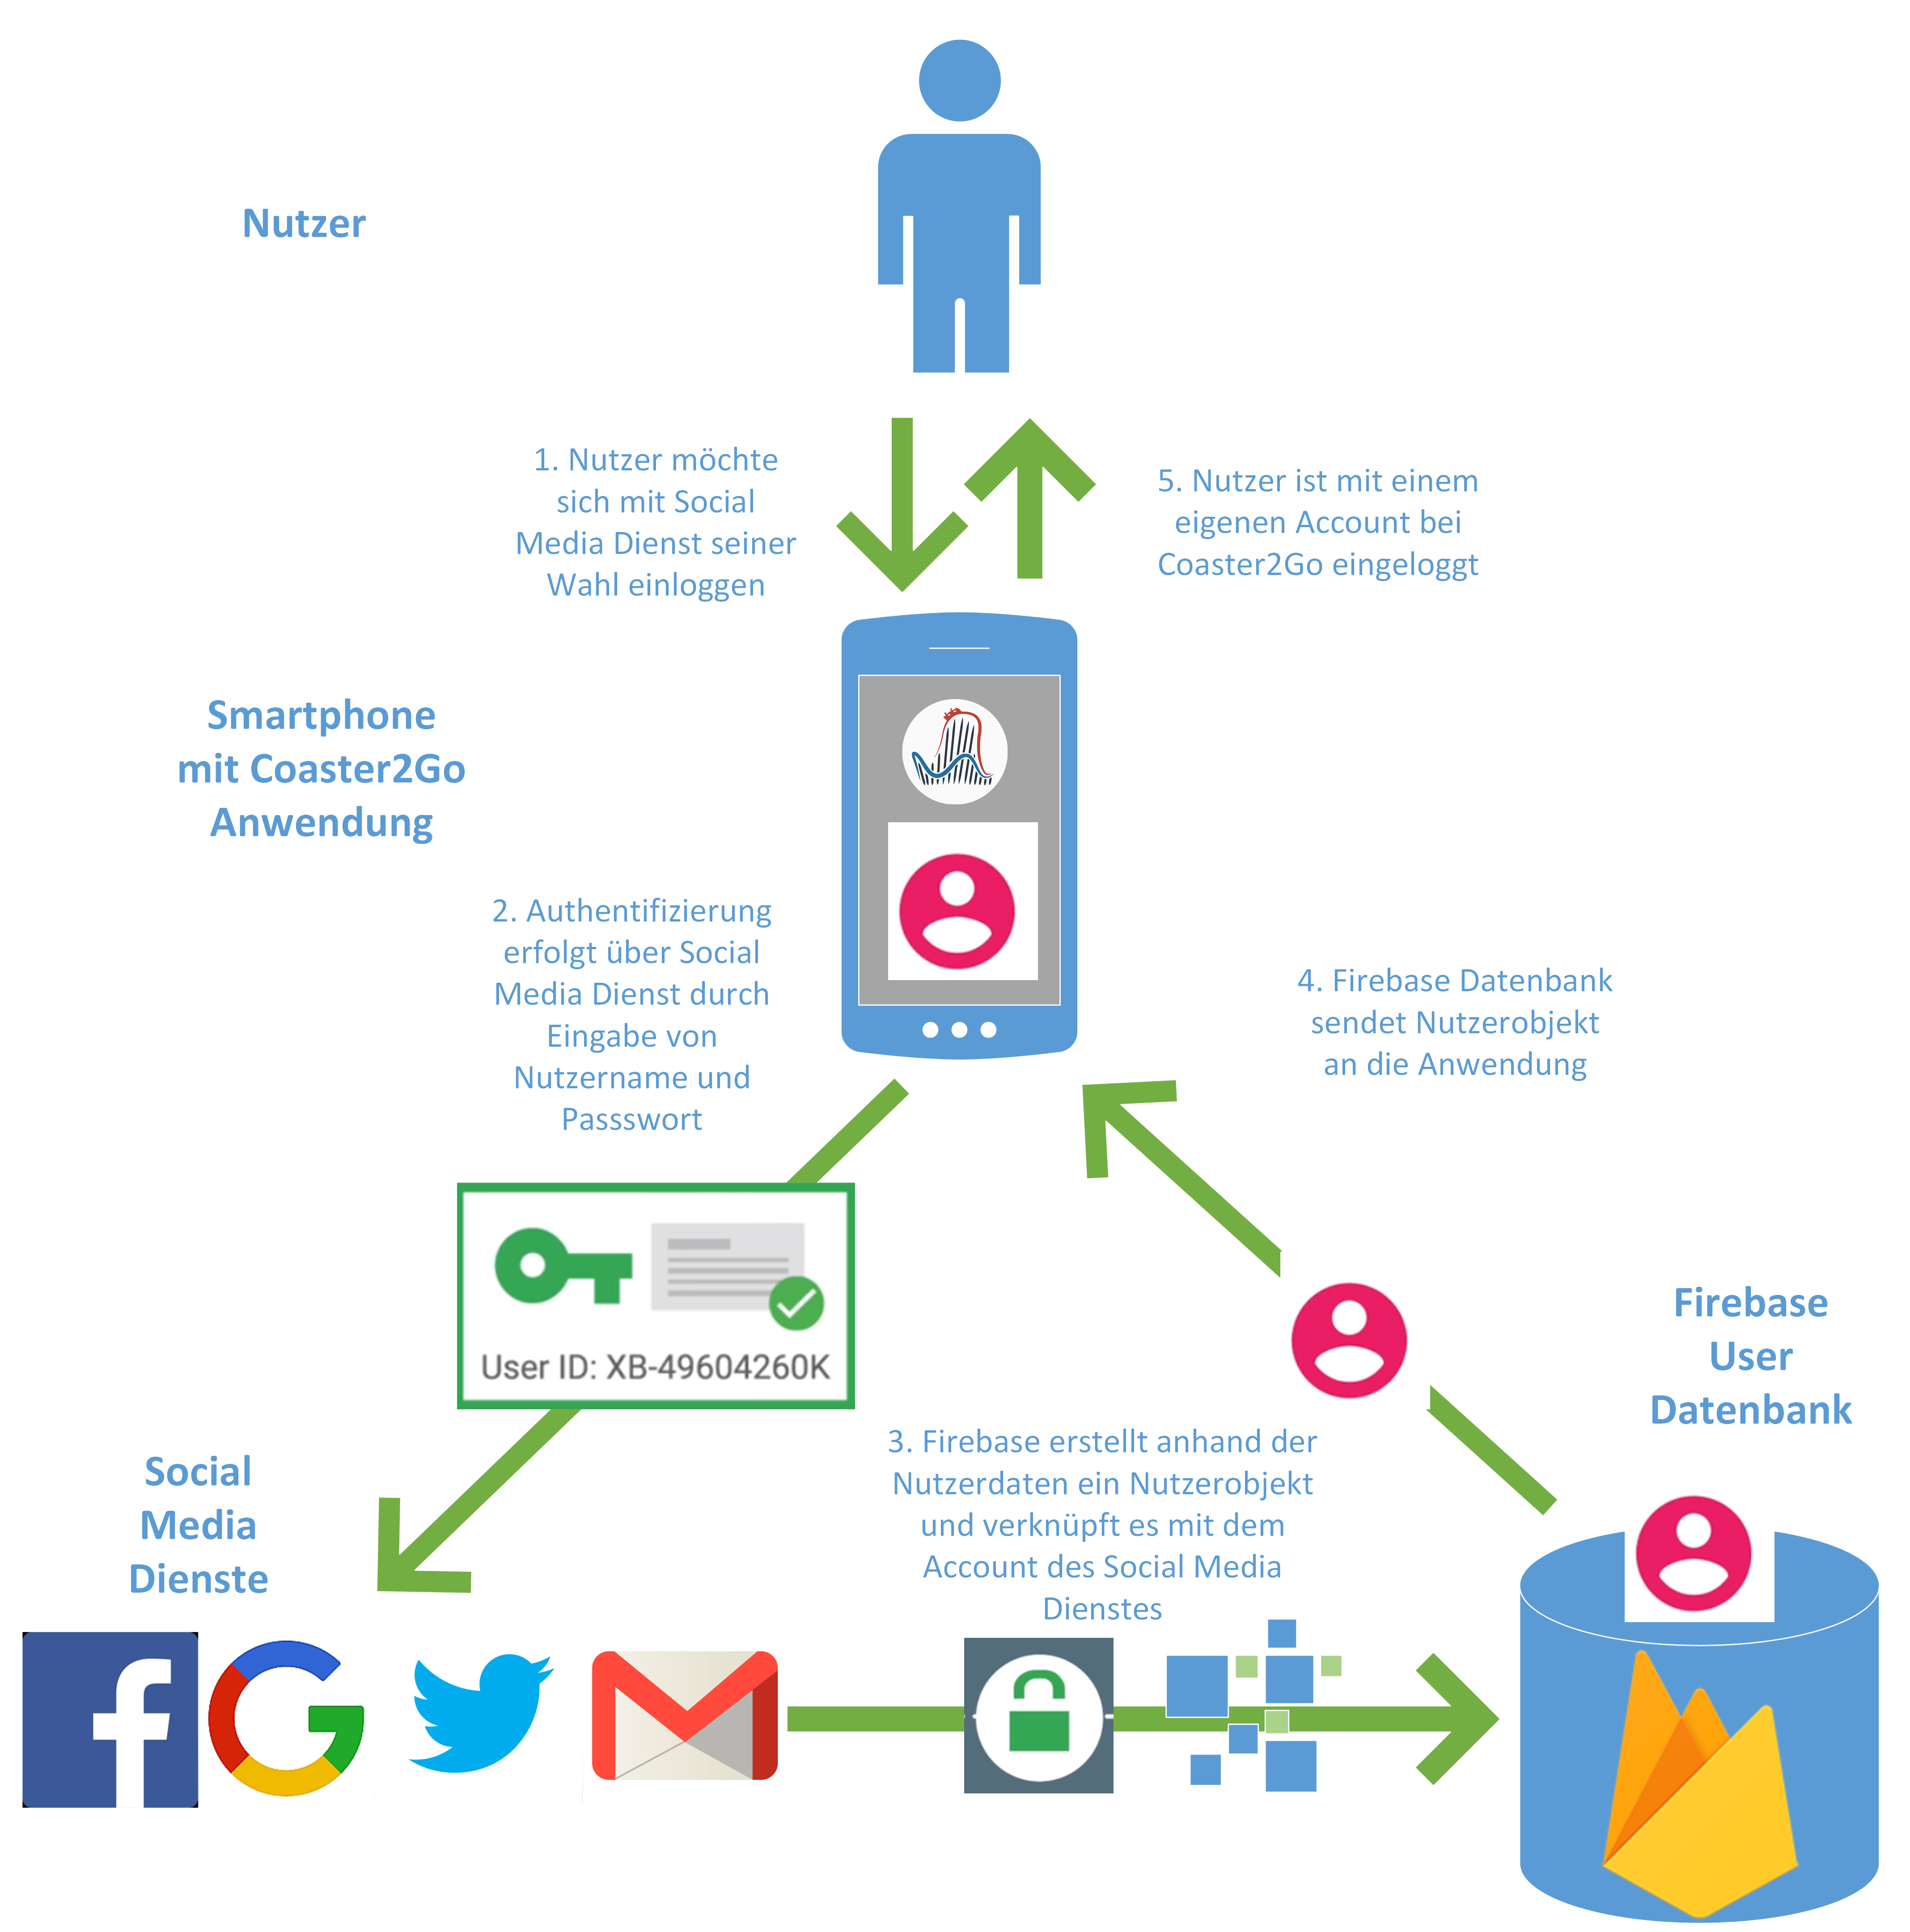
\includegraphics[width=0.99\textwidth]{img/modelle/firebase_modell.png}
	\caption{Firebase Nutzerverwaltung Modell}
	\label{figure:besonderheitenFirebase}
\end{figure}

Firebase bietet den Vorteil, dass es einem sämtliche Arbeiten im Bereich der Nutzerverwaltung abnimmt und man sich selbst nicht mehr groß damit beschäftigen muss. Der größte Vorteil ist auf jeden Fall die Einbindung der vielen anderen Social Media Dienste. Ein Nachteil sind die oft langen Ladezeiten beim Einloggen sowie ein reisen Overhead an benötigten Bibliotheken und Ressourcen für eine eigentlich nicht aufwendige Aufgabe.

% Abschnitt: Architektur
\section{Architektur}
\label{sec:implementierung:architektur}

\subsection{Datenmodell und -speicherung}
\label{sec:implementierung:architektur:datenmodell}

%Daten Modell
\begin{figure}[htp]
	\centering
  	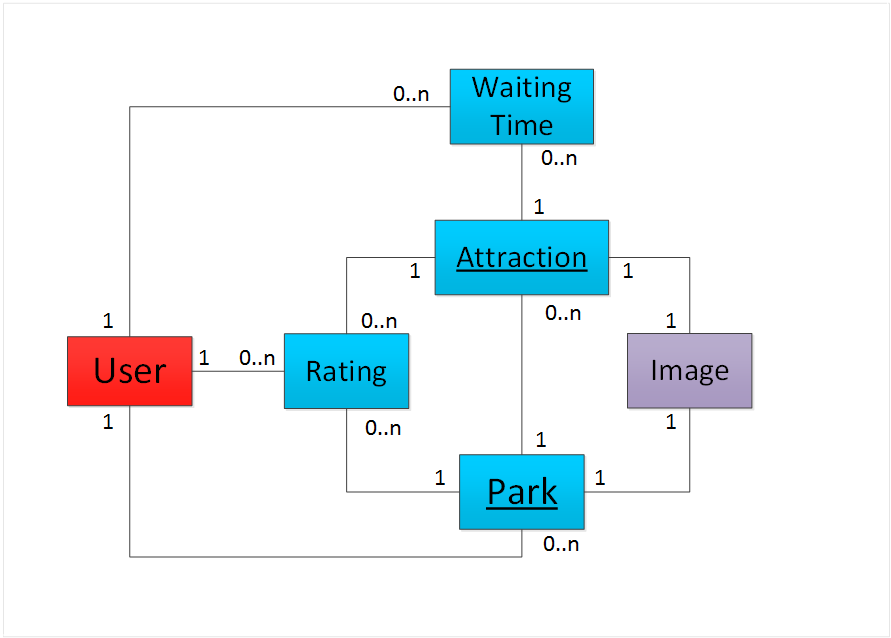
\includegraphics[width=0.99\textwidth]{img/modelle/Datenmodell.png}
	\caption{Datenmodell}
	\label{figure:architketurDatenmodell}
\end{figure}

In Abbildung \ref{figure:architketurDatenmodell} ist das Datenmodell für unsere App zu sehen. Es ist in diesem Fall nicht besonders kompliziert. Deswegen haben wir auch auf die Darstellung der einzelnen Attribute verzichtet, da diese sich implizit aus der Anwendungslogik ergeben. Die verschiedenen Farben sollen den Speicherort der Daten unterscheiden. Alle blauen Entitäten werden in Form von Tabellen in einer SQLite Datenbank auf einem Mircosoft Azure Server gespeichert. Die User-Daten werden von Firebase auf einem Firebase Server gespeichert. Und die Bilder werden über Cloudinary gespeichert. Der Grund hierfür ist zum einen, dass wir mit einem Studentenaccount keine Dateien bei Azure speichern können, und zum anderen, dass über Clourinary Bilder ganz einfach über einen Http-Request geladen und gleich auch noch transformiert werden können. Die Daten der beiden unterstrichenen Objekte (Attraction und Park) werden zusätzlich auch auf dem Handy in Form von JSON-Dateien gespeichert.

\subsection{Klassen- und Activity-Architektur}
\label{sec:implementierung:architektur:klassenmodell}

%Activity Modell
\begin{figure}[htp]
	\centering
  	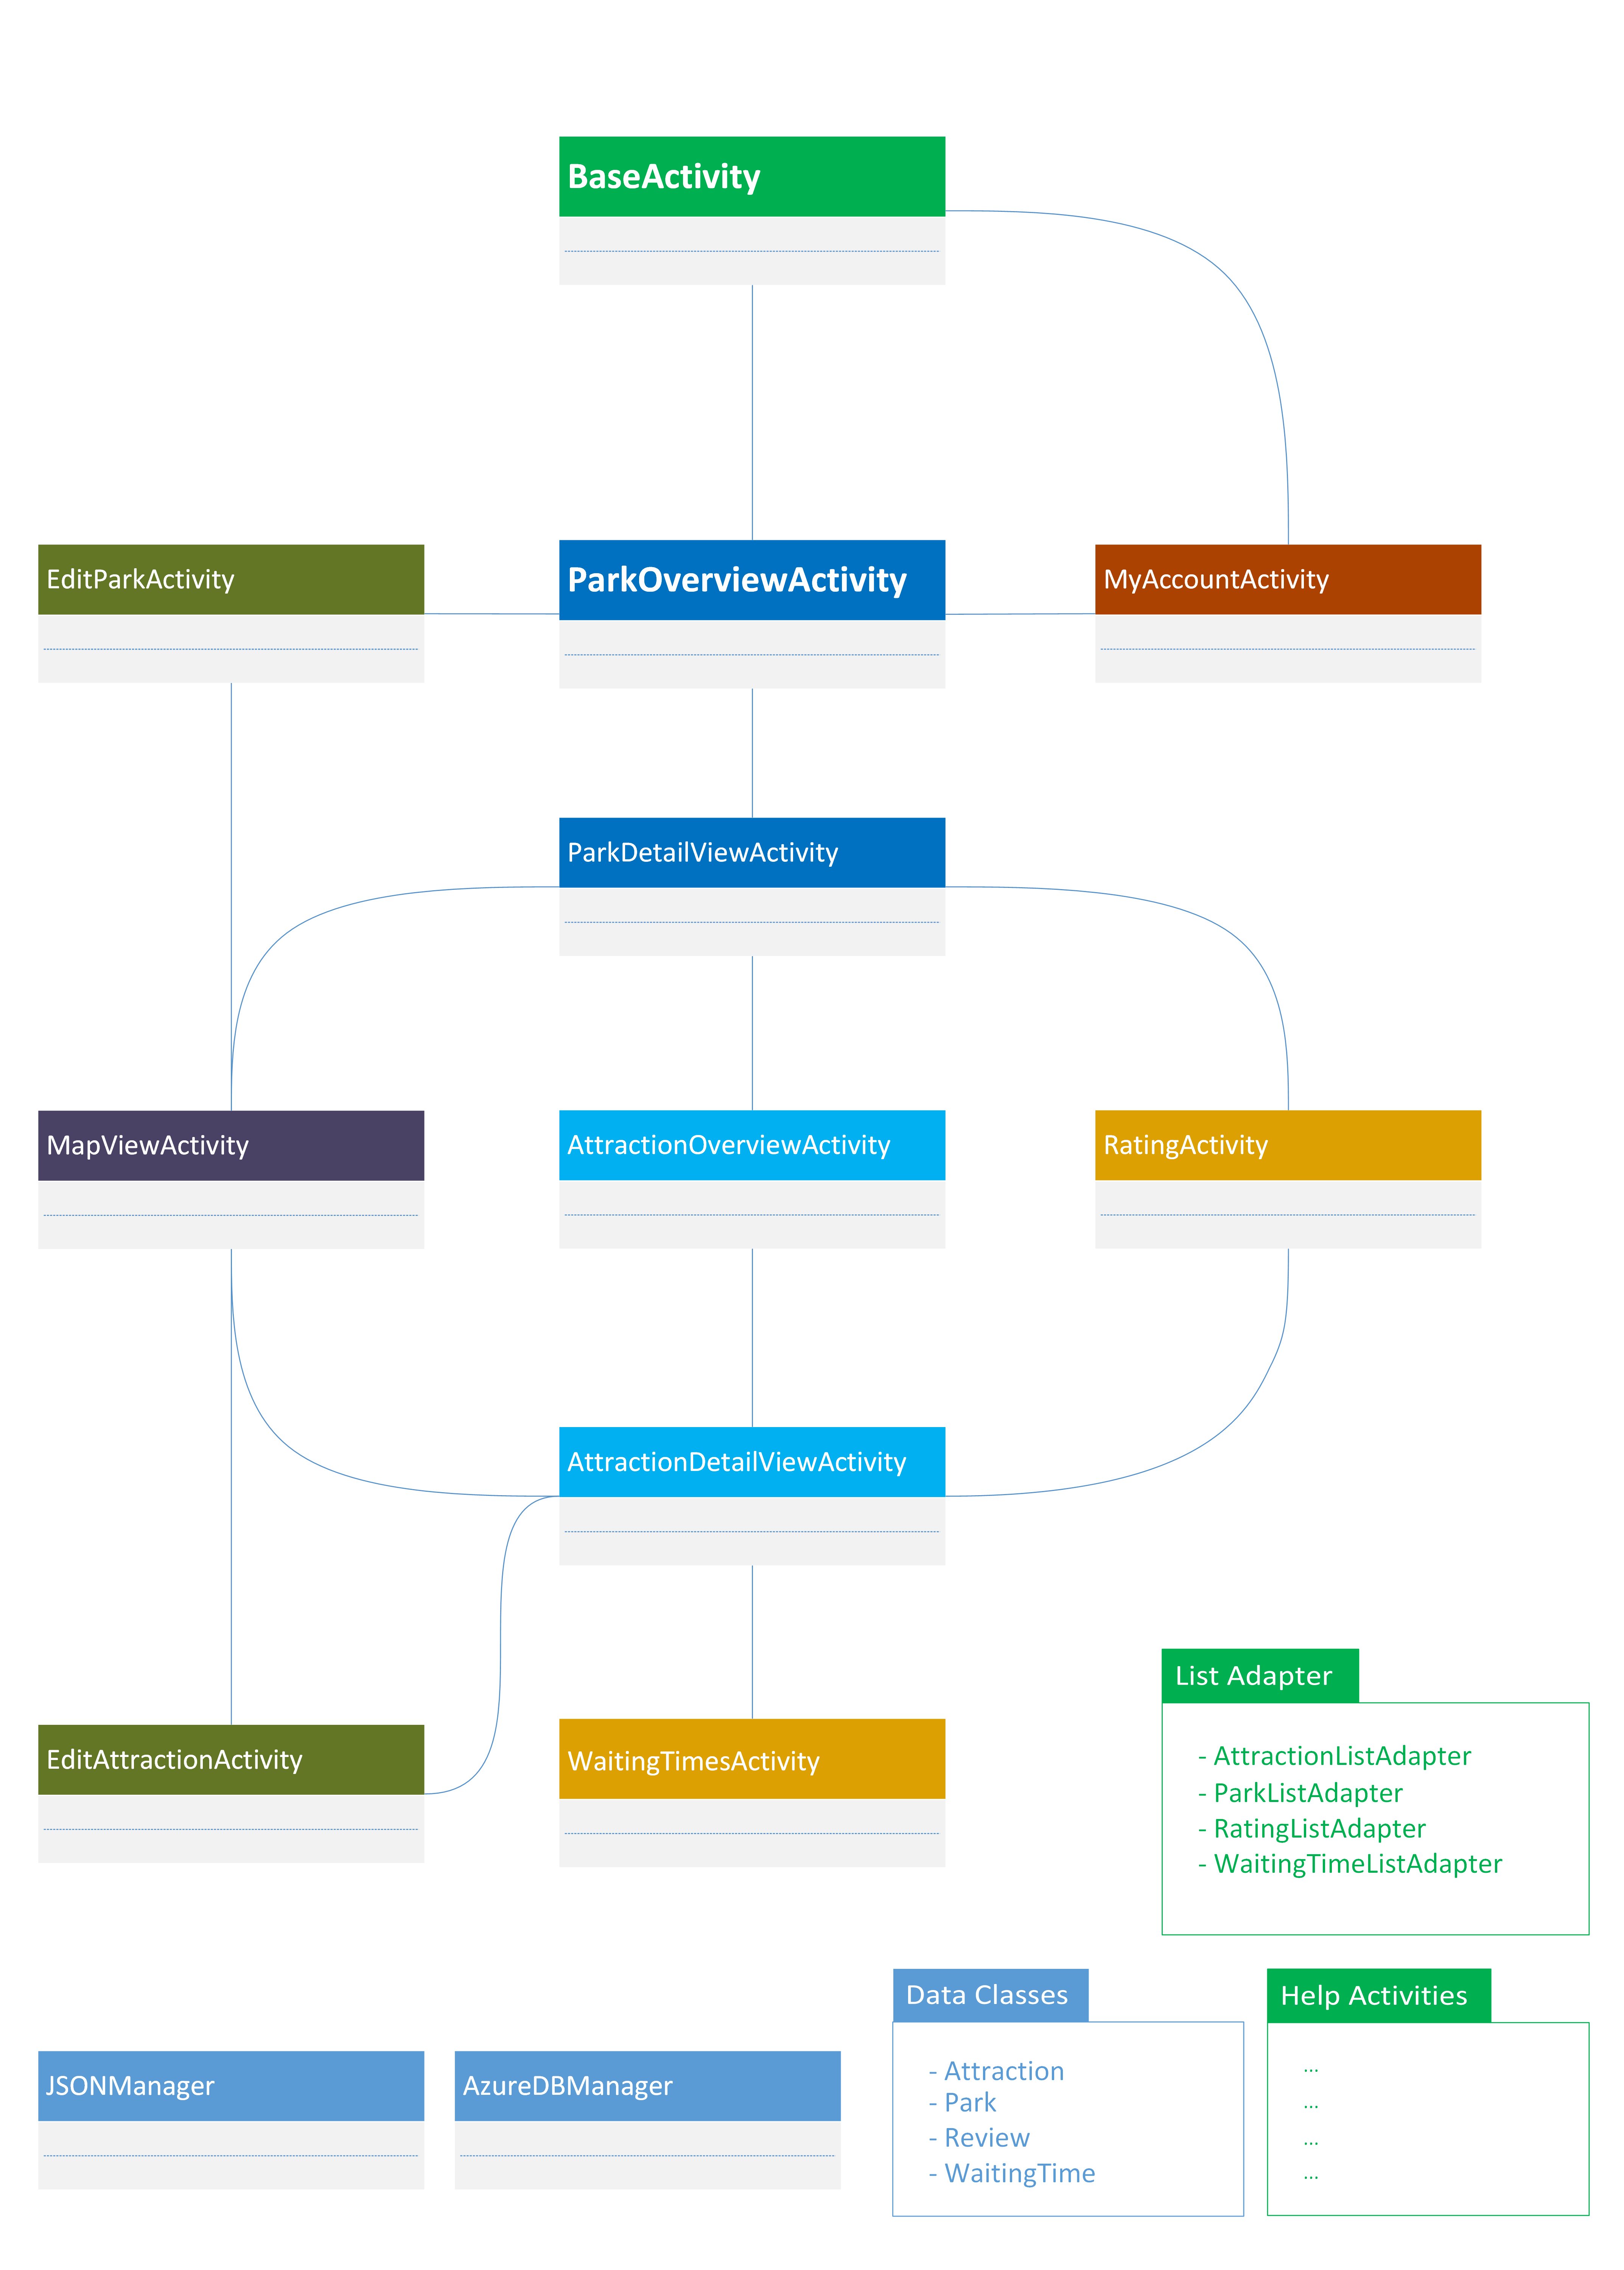
\includegraphics[width=0.99\textwidth]{img/modelle/Klassenmodell.png}
	\caption{Klassenmodell}
	\label{figure:architketurKlassenmodell}
\end{figure}

In Abbildung \ref{figure:architketurKlassenmodell} sieht man das Klassenmodell bzw. das Activity-Modell unserer App. Dort sind die einzelnen Activities und damit gleichzeitig Views unserer App und deren Verknüpfungen dargestellt. Die unterschiedlichen Farben sollen die Art der Activities symbolisieren. Die BaseActivity ist die Grund-Activity, von der alle anderen Activites erben, und auf die jederzeit zugegriffen werden kann. Die ParkOverviewActivity ist die Activity, die der Nutzer sieht, wenn er die App startet. Zusätzlich zu den Activities gibt es noch die Datenklassen, Klassen für die Onlinekommunikation und Offilnespeicherung der Daten, sowie einige Helferklassen und Klassen für Listadapter.

\subsection{Arbeitsaufteilung}
\label{sec:implementierung:architektur:arbeitsaufteilung}

Während der Implementation wurden die Aufgaben so aufgeteilt, dass jeder aus dem Team immer für eine bestimmte Aufgabe zuständig war und diese durch alle Schichten durch erledigen musste. Bei großen Aufgaben, wie den Übersichten oder den Detailansichten, wurden die Aufgaben zudem in kleinere Schritte aufgeteilt. Da die App aus mehreren unabhängigen Bereichen besteht, konnten die Aufgaben gut eingeteilt werden, ohne dass es zu Behinderungen kommt. Wenn gerade keine Arbeit für eine Person angefallen war, beschäftigte diese sich mit Verbesserungen, Testen von Funktionen oder mit der Weiterentwicklung des Designs.

% Abschnitt: Schwierigkeiten während der Implementierung 
\section{Herausforderungen während der Implementierung}
\label{sec:implementierung:schwierigkeiten}	

In diesem Abschnitt möchten wir noch auf einige Herausforderungen und Probleme eingehen, die wir während der Implementierung hatten, und wie wir diese gelöst haben. Generell muss man dazu sagen, dass es insgesamt doch zu deutlich weniger Problemen gekommen ist, als wir anfangs vermutet hatten. Und wenn Probleme aufkamen, hat man dank der ausführlichen Dokumentation und dank vielen Hilfen im Internet relativ schnell die Lösung dafür gefunden.

\begin{itemize} 
\item Unterstützung älterer Versionen bei Benutzung neuer Funktionen: Für fast alles gibt es bei Android mittlerweile bereits implementierte Funktionen, jedoch sind viele dieser Funktionen erst ab einer bestimmten Version verfügbar. Da wir unsere App aber explizit auch für ältere Android Modelle kompitabel machen wollten, mussten wir öfter die einfachere Variante außen vor lassen und etwas selbst implementieren.
\item Dex-Limit bei Android oder auch genannt das 64k Methoden-Limit: Dieses Limit taucht auf, wenn die App insgesamt mit allen Bibliotheken über 64.000 Methoden besitzt und auch mit älteren Android-Versionen kompitabel sein soll. Die vielen Methoden kommen dadurch zustande, wenn man mehrere Bibliotheken einbindet, die selbst widerum abhängig zu anderen Bibliotheken sind. So hat zum Beispiel alleine die Google-Play-Bibliothek über die Hälfte der Methoden ausgefüllt. Oft ist es so, dass nur eine Funktion einer Bibliothek gebraucht wird, sie aber komplett eingebunden werden muss. So haben wir trotz nicht all zu vieler Einbindungen recht schnell dieses Limit überschritten. Mit ein wenig Recherche konnte aber auch dieses Problem umgangen werden.
\item  Interface-Design so umsetzen wie geplant: Wie auch schon im letzten Semester kann man festhalten, dass das Designen der GUI mit Android Studio sehr angenehm ist. Trotzdem hat es uns erneut vor eine Herausforderung gestellt, die GUI auch so umzustzen wie geplant. Es gab alleine zwsichen unseren Handys und Emulatoren öfter mal größere Unterschiede bei der Darstellung.
\item Microsoft Azure: Azure bietet zwar viele Vorteile aber auch einige Schwierigkeiten, wie ein nicht intuitives Webinterface, Einschränkungen für Studenten und einen scheinbar zwischenzeitlich zufälligen sehr langsamen Verbindungsaufbau.
\item Möglichst wenige Verbindungen zum Server aufbauen: Die Daten schlau herunter zu laden und zwischen zu speichern, so dass der Client möglichst wenig Anfragen an den Server schicken muss, war nicht immer selbstverständlich. Es muss oft abgeschätzt werden, wann eine Anfrage an den Server sinnvoll ist und wann auf zwischengespeicherte Daten zurück gegriffen werden kann.
\item Benutzung von Google-Services: Das Arbeiten mit bereits vorhandenen APIs wie zum Beispiel den Maps- / Standort-Services musste erst erlernt werden. Aber dank der guten Dokumentation war dies kein Problem.
\end{itemize}